\documentclass[nochap]{apuntes}
\title{Autómatas y Lenguajes: Hoja 1}
\author{Pedro Valero}
\date{}

% Paquetes adicionales
\usepackage{tikztools}
\usepackage{fastbuild}
\usetikzlibrary{arrows}

\begin{document}
\pagestyle{plain}

%%%%%%%%%%%%%%%%%%%%%%%%%%%%%%%%%%%%%%%%%%%%%%%
%%%
%%% 		Problema 1
%%%
%%%%%%%%%%%%%%%%%%%%%%%%%%%%%%%%%%%%%%%%%%%%%%%
\begin{problem}
Sea la siguiente gramática:
\begin{itemize}
\item S ::= A
\item S ::= B
\item A ::= cA+b
\item A ::= a
\item B ::= cB+a
\item B :== b
\end{itemize}
 Calcula los conjuntos primero y siguiente para cada símbolo no terminal
\solution
\textbf{Primeros:}

\begin{itemize}
\item Primero(A) =$\{c,a\}$
\item Primero(B) =$\{c,b\}$
\item Primero(S) =$\{a,c,b\}$
\end{itemize}

\textbf{Sigueintes}

\begin{itemize}
\item siguiente(A) =$\{\$,+\}$
\item siguiente(B) =$\{\$, +\}$
\item siguiente(S) =$\{\$\}$
\end{itemize}
\end{problem}

%%%%%%%%%%%%%%%%%%%%%%%%%%%%%%%%%%%%%%%%%%%%%%%
%%%
%%% 		Problema 2
%%%
%%%%%%%%%%%%%%%%%%%%%%%%%%%%%%%%%%%%%%%%%%%%%%%
\begin{problem}
Sea la siguiente gramática LR(0):
\begin{itemize}
\item E ::= T
\item E ::= E + T
\item T ::= i
\item T ::= (E)
\end{itemize}
Calcula el cierre de la configuración inicial: E' ::= .ES
\solution
\begin{itemize}
\item E' ::= .ES
\item E ::= .T
\item E ::= .E + T
\item T ::= .i
\item T ::=.(E)
\end{itemize}
\end{problem}

%%%%%%%%%%%%%%%%%%%%%%%%%%%%%%%%%%%%%%%%%%%%%%%
%%%
%%% 		Problema 3
%%%
%%%%%%%%%%%%%%%%%%%%%%%%%%%%%%%%%%%%%%%%%%%%%%%
\begin{problem}
Sea la siguiente gramática LR(0):
\begin{itemize}
\item E ::= (L)
\item E ::= i
\item L ::= L,E
\item L ::= E
\end{itemize}

\ppart Calcula el cierre de la configuración E ::= (.L)

\ppart Calcula el estado al que se llega desde el estado anterior tras conocer el símbolo no terminal L.
\solution
\ppart
\begin{itemize}
\item E ::= (.L)
\item L ::= .L,E
\item L ::= .E
\item E ::= .(L)
\item E ::= .i
\end{itemize}

\ppart
\begin{itemize}
\item E ::= (L.)
\end{itemize}
puesto que el punto se encuentra delante de símbolos terminales no es necesario cerrar la configuración.
\end{problem}

%%%%%%%%%%%%%%%%%%%%%%%%%%%%%%%%%%%%%%%%%%%%%%%
%%%
%%% 		Problema 4
%%%
%%%%%%%%%%%%%%%%%%%%%%%%%%%%%%%%%%%%%%%%%%%%%%%
\begin{problem}
Sea la siguiente gramática

\begin{itemize}
\item D ::= iPSn
\item P ::= :n
\item S ::= λ
\item S ::= n
\end{itemize}

\ppart Dibuja el diagrama de estados del analizador LR(0) para dicha gramática
\ppart Calcula la tabla de análisis para el analizador LR(0)
\ppart Indica justificadamente si la gramática es LR(0). Indica justificadamente si es SLR(1)
\solution
Para trabajar con esta gramática primero añadimos la regla: D' ::= D\$, con lo que nos queda el conjunto de reglas:
\begin{itemize}
\item (0) D' ::= .D\$
\item (1) D ::= .iPSn
\item (2) P ::= .:n
\item (3) S ::= .λ
\item (4) S ::= .n
\end{itemize}
\ppart
\begin{center}
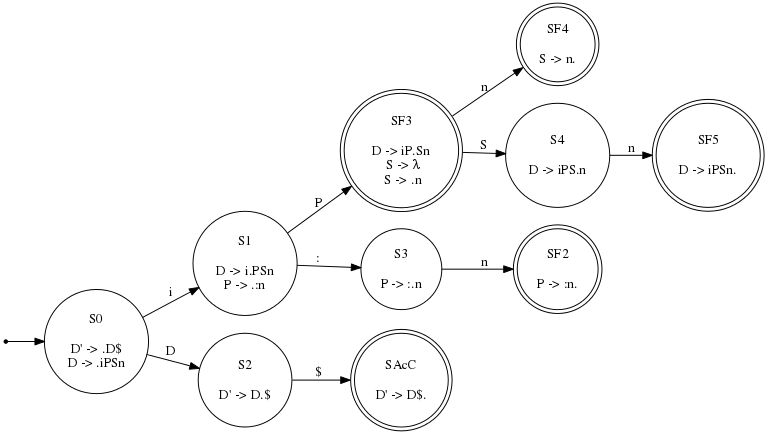
\includegraphics[scale=0.65]{automata_H3E4.png}
\end{center}

\ppart
\begin{tabular}{| c | c | c | c | c | c | c | c | }
\hline
Estado & i & n & : & \$ & D & P & S\\
\hline
S0 & d1 & &  &  & 2 &  & \\
\hline
S1 &  &  & d3 &  &  & F3 & \\
\hline
S2 &  &  &  & dacc &  & F5 &\\
\hline
SF3 & r3 & \textcolor{red}{r3/df4} & r3 & r3 &  &  & 4\\
\hline
S3 &  & dF2 & &  &  &  & \\
\hline
SF4 & r4  & r4  & r4 & r4 & &  &\\
\hline
S4 &  & dF5 &  &  &  &  & \\
\hline
SF2 & r2 & r2 & r2 & r2 &  &  & \\
\hline
SF5 & r1 & r1 & r1 & r1 &  &  & \\
\hline
\end{tabular}
\ppart \textbf{No se trata de una gramática LR(0)} ya que hay ocasiones en las que observamos un conflico desplazamiento-reducción. Por ejemplo, en el estado inicial podemos reducir la S o desplazar según la entrada dada.

Para ver si se trata de una gramática SLR(1) vamos a ver si somos capaces de solucionar los conflictos sabiendo cuales son los elementos siguientes:
\begin{itemize}
\item siguiente(D)={\$} : solo reducimos la regla 1 si después hay un '\$'.
\item siguiente(P)={n} : solo reducimos la regla 2 si después hay una 'n'.
\item siguiente(S)={n} : solo reducimos las reglas 3 y 4 si después hay una 'n'.
\end{itemize}

Sin embargo, \textbf{tampoco se trata de una gramática SLR(1)} ya que si forzamos a que las reducciones se produzcan en presencia del siguiente elemento no evitamos el conflicto. Como el siguiente de S es n, en presencia de esta n podremos aplicar la reducción S ::= λ o desplazar según la regla S ::= n. Quedando la siguiente tabla SLR(1):

\begin{tabular}{| c | c | c | c | c | c | c | c | }
\hline
Estado & i & n & : & \$ & D & P & S\\
\hline
S0 & d1 & &  &  & 2 &  & \\
\hline
S1 &  &  & d3 &  &  & F3 & \\
\hline
S2 &  &  &  & dacc &  & F5 &\\
\hline
SF3 &  & \textcolor{red}{r3/df4} &  &  &  &  & 4\\
\hline
S3 &  & dF2 & &  &  &  & \\
\hline
SF4 &   & r4  &  &  & &  &\\
\hline
S4 &  & dF5 &  &  &  &  & \\
\hline
SF2 &  & r2 &  &  &  &  & \\
\hline
SF5 &  &  &  & r1  &  &  & \\
\hline
\end{tabular}

\end{problem}

%%%%%%%%%%%%%%%%%%%%%%%%%%%%%%%%%%%%%%%%%%%%%%%
%%%
%%% 		Problema 5
%%%
%%%%%%%%%%%%%%%%%%%%%%%%%%%%%%%%%%%%%%%%%%%%%%%
\begin{problem}
Sea la siguiente gramática:
\begin{itemize}
\item S ::= bLd
\item L ::= E;L
\item L ::= λ
\item E ::= i=c
\item E ::= b
\end{itemize}
\ppart Dibuja el diagrama de estados del analizador LR(0) para dicha gramática
\ppart Calcula la tabla de análisis para el analizador LR(0)
\ppart Indica justificadamente si es SLR(1)

\solution
\ppart Extendemos la gramática para realizar el análisis LR(0):

\begin{itemize}
\item (0) S' ::= S \$
\item (1) S ::= bLd
\item (2) L ::= E;L
\item (3) L ::= λ
\item (4) E ::= i=c
\item (5) E ::= b
\end{itemize}
\begin{center}
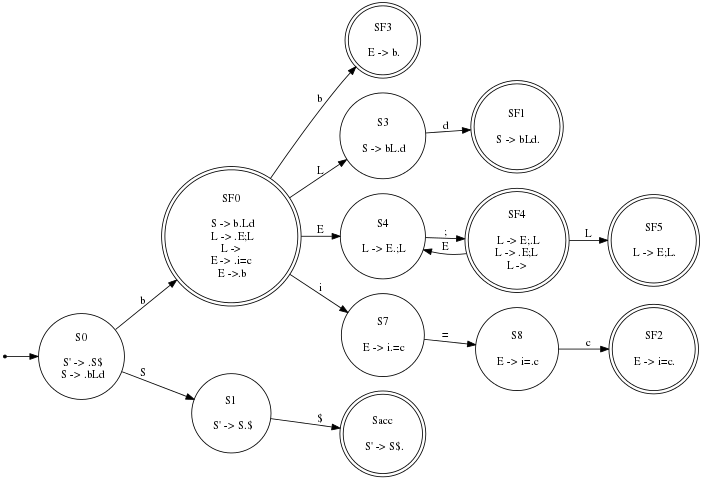
\includegraphics[scale=0.65]{automata5.png}
\end{center}

\ppart
\begin{tabular}{| c | c | c | c | c | c | c | c | c | c | c | }
\hline
Estado  & i & = & c & ; & b & d & \$ & L & E & S \\
\hline
S0 &  &  &  &  & dF0 &  &  &  &  & 1\\
\hline
S1 &  &  &  &  &  &  & dacc &  &  & \\
\hline
SF0 & \textcolor{red}{r3/d7} & r3 & r3 & r3 & \textcolor{red}{r3/dF3} & r3 & r3 & 3 & 4 & \\
\hline
S3 &  &  &  &  &  & dF1 &  &  &  & \\
\hline
SF1 & r1 & r1 & r1 & r1 & r1 & r1 & r1 &  &  & \\
\hline
S4 &  &  &  & dF4 &  &  &  &  &  & \\
\hline
SF4 & r3 & r3 & r3 & r3 & r3 & r3 & r3 & F5 & 4 & \\
\hline
SF5 & r2 & r2 & r2 & r2 & r2 & r2 & r2 &  &  & \\
\hline
SF3 & r5 & r5 & r5 & r5 & r5 & r5 & r5 &  &  & \\
\hline
S7 &  & d8 &  &  &  &  &  &  &  & \\
\hline
S8 &  &  & dF2 &  &  &  &  &  &  & \\
\hline
SF2 & r4 & r4 & r4 & r4 & r4 & r4 & r4 &  &  & \\
\hline
\end{tabular}
\ppart \textbf{No se trata de una gramática LR(0)} ya que hay ocasiones en las que observamos un conflicto desplazamiento-reducción. 

Para ver si se trata de una gramática SLR(1) vamos a ver si somos capaces de solucionar los conflictos sabiendo cuales son los elementos siguientes:
\begin{itemize}
\item siguiente(L)={d} : solo reducimos las reglas 2 y 3 si después hay una 'd'.
\item siguiente(E)={;} : solo reducimos las reglas 4 y 5 si después hay un ';'.
\item siguiente(S)={\$} : solo reducimos la regla 1 si después hay un '\$'.
\end{itemize}

Se corrigen los dos conflictos que hay ya que en el estado SF0 solo reduciremos si llega una 'd', por tanto en el caso de que llegue una 'b' o una 'i' desplazaremos. Quedando la tabla así:

\begin{tabular}{| c | c | c | c | c | c | c | c | c | c | c | }
\hline
Estado  & i & = & c & ; & b & d & \$ & L & E & S \\
\hline
S0 &  &  &  &  & dF0 &  &  &  &  & 1\\
\hline
S1 &  &  &  &  &  &  & dacc &  &  & \\
\hline
SF0 & d7 &  &  &  & dF3 & r3 &  & 3 & 4 & \\
\hline
S3 &  &  &  &  &  & dF1 &  &  &  & \\
\hline
SF1 &  &  &  &  &  &  & r1 &  &  & \\
\hline
S4 &  &  &  & dF4 &  &  &  &  &  & \\
\hline
SF4 &  &  &  &  &  & r3 &  & F5 & 4 & \\
\hline
SF5 &  &  &  &  &  & r2 &  &  &  & \\
\hline
SF3 &  &  &  & r5 &  &  &  &  &  & \\
\hline
S7 &  & d8 &  &  &  &  &  &  &  & \\
\hline
S8 &  &  & dF2 &  &  &  &  &  &  & \\
\hline
SF2 &  &  &  & r4 &  &  &  &  &  & \\
\hline
\end{tabular}

\end{problem}

%%%%%%%%%%%%%%%%%%%%%%%%%%%%%%%%%%%%%%%%%%%%%%%
%%%
%%% 		Problema 6
%%%
%%%%%%%%%%%%%%%%%%%%%%%%%%%%%%%%%%%%%%%%%%%%%%%
\begin{problem}
Calcula los conjuntos primero y siguiente de todos los símbolos no terminales de las gramáticas siguientes

\ppart
\begin{itemize}
\item X ::= Ye
\item X ::= eYZf
\item Y ::= g
\item Y ::= Yg
\item Z ::= h
\end{itemize}

\ppart
\begin{itemize}
\item Q ::= fXY
\item X ::= cQ
\item X ::= λ
\item Y ::= iQ
\item Y ::= λ
\end{itemize}

\ppart
\begin{itemize}
\item A ::= BXB
\item X ::= ,
\item X ::= .
\item X ::= e
\item B ::= 0B
\item B ::= 1B
\item B ::= λ
\end{itemize}

\solution
\ppart
\begin{itemize}
\item primero(X)=\{e,g\}
\item primero(Y)=\{g\}
\item primero(Z)=\{h\}
\end{itemize}
\begin{itemize}
\item siguiente(X)=\{\$\}
\item siguiente(Y)=\{\$,e,h\}
\item siguiente(Z)=\{\$,f\}
\end{itemize}

\ppart
\begin{itemize}
\item primero(X)=\{c,i,f\}
\item primero(Y)=\{i,f\}
\item primero(Q)=\{f\}
\end{itemize}
\begin{itemize}
\item siguiente(X)=\{\$,i,f\}
\item siguiente(Y)=\{\$,i,f\}
\item siguiente(Q)=\{\$,i,f\}
\end{itemize}

\ppart
\begin{itemize}
\item primero(X)=\{",",.,e\}
\item primero(A)=\{0,1,",",.,e\}
\item primero(B)=\{0,1,",",.,e\}
\end{itemize}
\begin{itemize}
\item siguiente(X)=\{\$,0,1\}
\item siguiente(A)=\{\$,\}
\item siguiente(B)=\{\$,",",.,e\}
\end{itemize}

\end{problem}

%%%%%%%%%%%%%%%%%%%%%%%%%%%%%%%%%%%%%%%%%%%%%%%
%%%
%%% 		Problema 7
%%%
%%%%%%%%%%%%%%%%%%%%%%%%%%%%%%%%%%%%%%%%%%%%%%%
\begin{problem}
Cacula los símbolos de adelanto para el cierre de las siguientes reglas y gramáticas:
\ppart Cierre de E' ::= .E $\{ \$ \}$ para la siguiente gramática
\begin{itemize}
\item E' ::= E
\item E ::= T
\item E ::= E+T
\item T ::= i
\item T ::= (E)
\end{itemize}

\ppart Cierre de S' ::= .s $\{ \$ \}$ para la siguiente gramática
\begin{itemize}
\item S' ::= S
\item S ::= L=R
\item S ::= R
\item L ::= *R
\item L ::= i
\item R ::= L
\end{itemize}

\ppart Cierre de E ::= (.E) $\{ \$ \}$ para la siguiente gramática
\begin{itemize}
\item E ::= (L)
\item E ::= a
\item L ::= L,E
\item L ::= E
\end{itemize}
\solution
\ppart
El cierre, con los conjuntos de adelanto, sería
\begin{itemize}
\item E' ::= .E $\{\$\}$
\item E ::= .T $\{\$\}$
\item E ::= .E+T $\{+,\$\}$
\item T ::= .i $\{+,\$\}$
\item T ::= .(E) $\{\$\}$
\end{itemize}

\ppart
\begin{itemize}
\item S' ::= .S $\{\$\}$
\item S ::= .L=R $\{\$\}$
\item S ::= .R $\{\$\}$
\item L ::= .*R $\{=, \$\}$
\item L ::= .i $\{=, \$\}$
\item R ::= .L $\{\$\}$
\end{itemize}

\ppart
\begin{itemize}
\item E ::= (.L) $\{\$\}$
\item L ::= .L,E $\{",", )\}$
\item L ::= .E $\{",", )\}$
\item E ::= .a $\{",", )\}$
\item E ::= .(L) $\{",", )\}$
\end{itemize}
\end{problem}

%%%%%%%%%%%%%%%%%%%%%%%%%%%%%%%%%%%%%%%%%%%%%%%
%%%
%%% 		Problema 8
%%%
%%%%%%%%%%%%%%%%%%%%%%%%%%%%%%%%%%%%%%%%%%%%%%%
\begin{problem}
Sea la siguiente gramática independiente del contexto:
\begin{itemize}
\item S ::= aSb
\item S ::= ab
\end{itemize}
\ppart Dibuja el diagrama de estados del analizador LR(1) para dicha gramática
\ppart Calcula la tabla de análisis para el analizador LR(1)
\ppart Usa la tabla de análisis para analizar la sentencia $aabb$
\ppart Dibuja esquemáticamente el diagrama de estados LALR(1). Es suficiente con indicar los nombres de los estados, especificando cuáles son la unión de otros en LR(1).
\solution
\ppart
\begin{center}
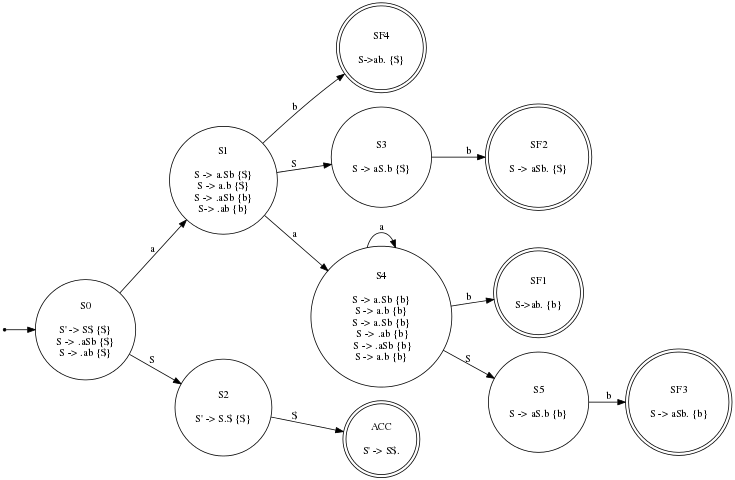
\includegraphics[scale=0.65]{automata_H3E8.png}
\end{center}

\ppart
\begin{tabular}{| c | c | c | c | c |}
\hline
Estado & S & a & b & \$\\
\hline
S0 & S2 & S1 & & \\
\hline
S1 & S3 & S4 & SF4 & \\
\hline
S2 & & & & ACC \\
\hline
S3 & & & SF2 & \\
\hline
S4 & S5 & S4 & SF1 & \\
\hline
S5 & & & SF3 & \\
\hline
SF1 & & & r3 & \\
\hline
SF2 & & & & r2\\
\hline
SF3 & & & r3 & \\
\hline
SF4 & & & & r3 \\
\hline
ACC & & & & r1 \\
\hline
\end{tabular}

\ppart
La secuencia de acciones sería la siguiente:
\begin{verbatim}
Cadena: .aabb / Leemos 'a' y pasamos a S1
Cadena: a.abb / Leemos 'a' y pasamos a S4
Cadena: aa.bb / Leemos b y pasamos a SF1
Cadena: aab.b / Como el siguiente elemento a leer es b reducimos y volvemos a S0
Cadena: .aSb / Leemos 'a' y pasamos a S1
Cadena: a.Sb / Leemos 'S' y pasamos a S3
Cadena: aS.b / Leemos 'b' y pasamos a SF2
Cadena: aSb. / Como el siguiente elemento a leer es $, reducimos y volvemos a S0
Cadena: .S / Leemos S y pasamos a S2
Cadena: . / Fin de cadena. Pasamos a ACC y aceptamos la entrada
\end{verbatim}

\ppart
Cuando pasemos de LR(1) a LALR(1) vamos a agrupar los nodos S3 y S5 en uno solo así como SF2 y SF3, manteniendo las mismas reglas en cada caso y estableciendo como símbolos de adelanto la unión de los símbolos de adelanto de las reglas de los estados a unir.
\end{problem}

%%%%%%%%%%%%%%%%%%%%%%%%%%%%%%%%%%%%%%%%%%%%%%%
%%%
%%% 		Problema 9
%%%
%%%%%%%%%%%%%%%%%%%%%%%%%%%%%%%%%%%%%%%%%%%%%%%
\begin{problem}
Sea la siguiente gramática independiente del contexto:
\begin{itemize}
\item S ::= XX
\item X ::= aX
\item X ::= b
\end{itemize}
\ppart Dibuja el diagrama de estados del analizador LR(1) para dicha gramática
\ppart Calcula la tabla de análisis para el analizador LR(1)
\ppart Usa la tabla de análisis para analizar la sentencia $aabb$
\ppart Dibuja esquemáticamente el diagrama de estados LALR(1). Es suficiente con indicar los nombres de los estados, especificando cuáles son la unión de otros en LR(1).
\solution
\ppart Extendemos la gramática para realizar el análisis LR(1):

\begin{itemize}
\item (0) S' ::= S
\item (1) S ::= XX
\item (2) X ::= aX
\item (3) X ::= b
\end{itemize}
\begin{center}
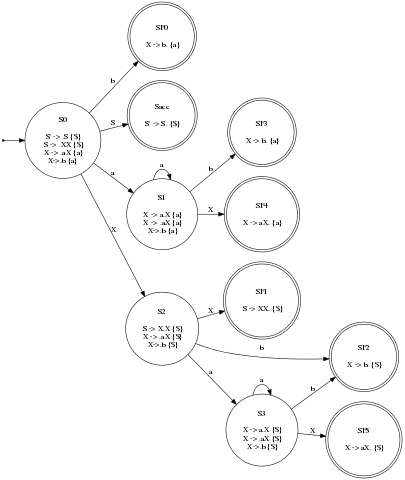
\includegraphics[scale=0.65]{automata9.png}
\end{center}

\ppart
\begin{tabular}{| c | c | c | c | c | }
\hline
Estado  & a & b & X & S \\
\hline
S0 & d1 & dF0 & acc & 2\\
\hline
SF0 & r3  & r3 &  & \\
\hline
S1 & d1 & dF3 & F4 &  \\
\hline
SF3 & r3 & r3 &  & \\
\hline
SF4 & r2 & r2 &  &   \\
\hline
S2 & d3 & dF2 & F1 &  \\
\hline
SF1 & r1 & r1 &  &  \\
\hline
S3 & d3 & dF2 & F5 & \\
\hline
SF5 & r2 & r2 &  &  \\
\hline
SF2 & r3 & r3 &  &  \\
\hline
\end{tabular}


\end{problem}

%%%%%%%%%%%%%%%%%%%%%%%%%%%%%%%%%%%%%%%%%%%%%%%
%%%
%%% 		Problema 10
%%%
%%%%%%%%%%%%%%%%%%%%%%%%%%%%%%%%%%%%%%%%%%%%%%%
\begin{problem}
Sea la siguiente gramática

\begin{itemize}
\item D ::= iPSn
\item P ::= :n
\item S ::= λ
\item S ::= n
\end{itemize}

\ppart Dibuja el diagrama de estados del analizador LR(1) para dicha gramática
\ppart Calcula la tabla de análisis para el analizador LR(1)
\ppart Indica justificadamente si la gramática es LR(1). Indica justificadamente si es SLR(1)
\solution
TODO
\end{problem}


\end{document}
